\subsection{Evaluation}

\subsubsection{Fetch time}
We implemented our search protocols based on BF-COIE, PS-COIE, and
BFS-CODE schemes. 
All protocols were implemented using PySEAL~\cite{pyseal}, which
is a Python wrapper of the Microsoft research SEAL library (version
3.6)~\cite{sealcrypto} using the BFV encryption scheme~\cite{BFV}.  We
instantiated a single-server PIR protocol in our construction using
SealPIR~\cite{SP:ACLS18}. For the root finding step of the decoding
procedure in PS-COIE, we use an implementation based on SageMath
9.2~\cite{Sage}.
 
\paragraph{Measuring the Fetch step.}
Our search framework improves the overall search time by executing the
Match step only once, while the LEAF protocol must execute the Match
step $s$ times. However, since we do not optimize the Match step itself
over prior work, we focus on measuring the cost of the Fetch procedure.
That is, our experiments measure the time from when the server holds
encrypted query results, i.e., $(\lbra b_1 \lket, \ldots, \lbra b_n
\lket)$ with $b_i \in \zo$, to when the client recovers all $s$ records
matching the query.  Specifically, we measure the cost of steps 4 and up
in Algorithms~\ref{alg:ssCOIE} and~\ref{alg:ssCODE}.  Similarly, for
LEAF+, we only measure the cost of the Fetch step.  

\paragraph{Database.}
To measure the performance of our protocols, we run experiments with
database size $n$ ranging from 1000 to 100,000 data items and the result
set size $s$ set to between 8 and 128.  As in the LEAF+
experiments~\cite{CCS:WYXZ20}, all data items are $16$-bit integers. 

\paragraph{BF-COIE parameters.}
For the BF-COIE secure search, we set the parameters as indicated in
Section~\ref{sec:BF-COIE}. 
\BI
\item 
We set the false positive upperbound $f_p = 16$.  Recall that the client
aborts (without executing the PIR) if the actual number of false
positives exceeds this, but this only happens with probability
negligible in the security parameter, which we set $\secparam = 40$.

\item We set the number of hash function $\eta=2$ for each Bloom filter, so
  each BF has size $\ell = 2s \cdot \sqrt{2s}$. (If $2s < s + 2f_p$, we set
  $\ell = 2s \cdot \sqrt{s + 2f_p}$). 
\EI

\paragraph{BFS-CODE parameters.}
For BFS-CODE secure search, with $\secparam = 40$, the number of
hash functions $\eta$ is set to $\secparam+\lg{s}$, and the Bloom filter
size is set to $2(\eta s - 1)$. 
%
Additionally, each data item is attached with a 40-bit checksum to
guarantee a $2^{-\secparam}$ probability of collision. We used SHA2 to
compute a checksum.   

\paragraph{Implementing LEAF+.}
For a comparison we also implemented the fetch step of the LEAF+
protocol~\cite{CCS:WYXZ20}, since their implementation is not publicly available.

Their protocol has $O(\log \log n)$ depth of multiplications. Therefore, they
have to use bootstrapping techniques to reduce the accumulated noise.
However, SEAL doesn't provide a method for bootstrapping, and we suspect
that they added a customized implementation of bootstrapping on top of
SEAL. Unfortunately, their implementation is not available. 

We address this issue by choosing to ignore the time for bootstrapping
when we measure the running time of our implementation of LEAF+. Of
course, our implementation doesn't output the correct results, but the
measured running time will be shorter than the actual running time.
Therefore, we believe that this measured time serves as a good baseline.  

\paragraph{Experiment environments.}
All our experiments were performed on an Intel\textregistered Core 9900k
@4.7GHz with 64GB of memory. For fair comparison, the test was performed
on a single thread with no batching optimizations for computation.
Networking protocol between server and clients is a 1Gbps LAN.
%which
%simulates the Gigabyte Connection bandwidth offered by Verizon FIOS.
%\anote{Need to say something about network.} \lins{Do we need any
%citation for verizon? }

% during computation.
%We used batching only when serializing the final ciphertexts to reduce
%the network communication. 


\begin{figure}
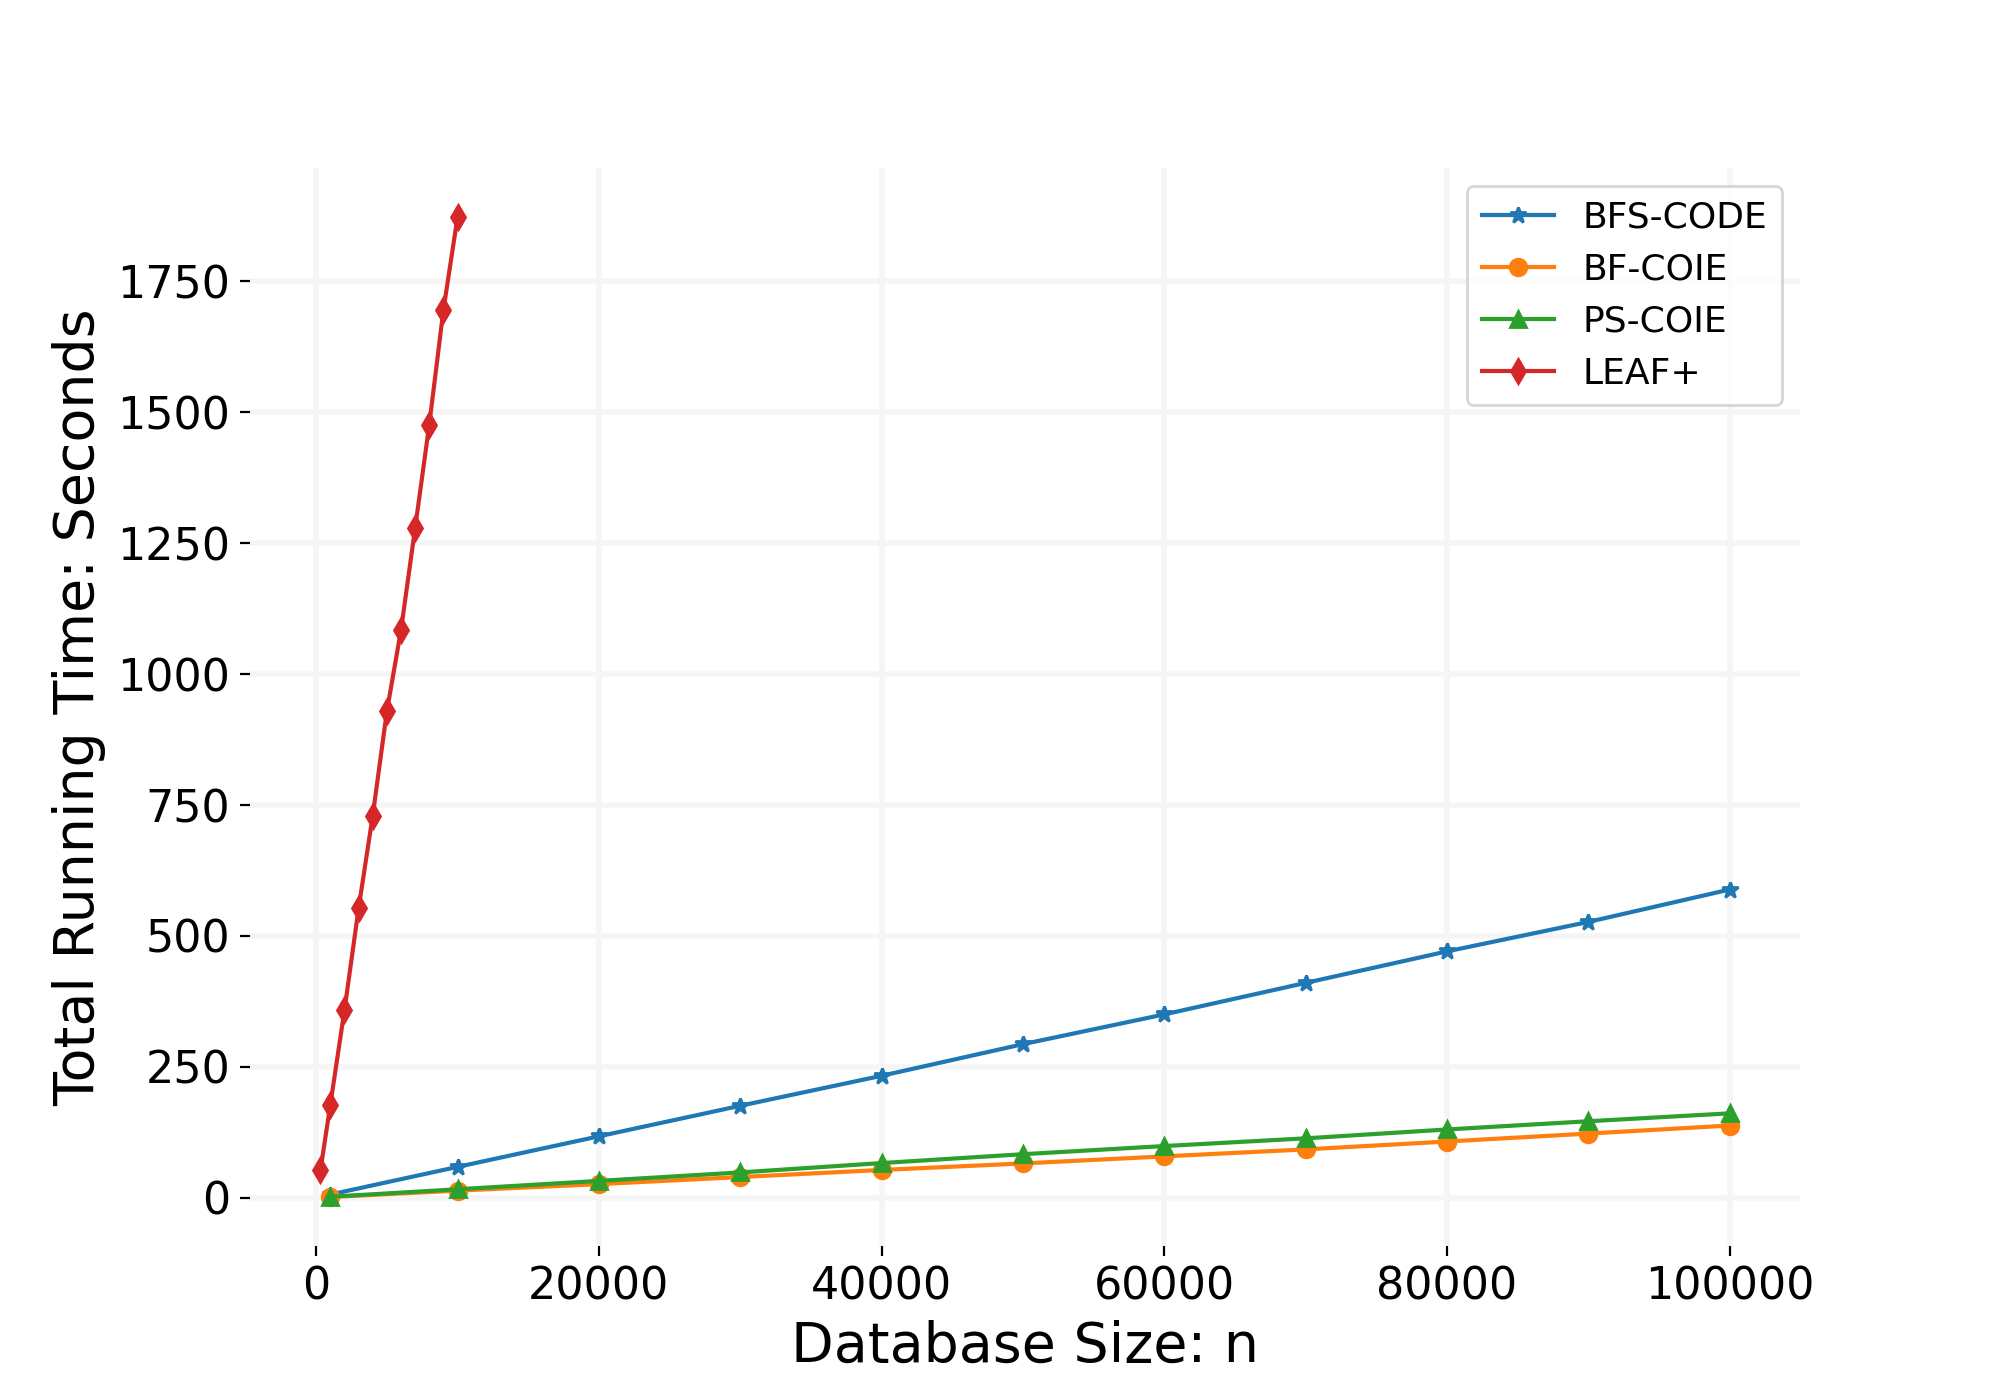
\includegraphics[width=.95\linewidth]{src/securesearch/expimgs/Figure_n.png}
\BI
\item[]
{\small For {LEAF+}, we plot the time for fetching only a {\bf
single} record, since fetching $s$ records takes too long.}
\EI
\caption{Fetch time vs. Database size with $s=16$.}
\label{fig:t_n}
\end{figure}

\paragraph{Results: Fetch time vs.~database size.}
Figure~\ref{fig:t_n} shows the performance of our protocols as a
function of database size, while the result set size $s$ is fixed to 16.
However, for {LEAF+}, we plot the time for fetching only a {\bf single}
record, since fetching $s$ records takes too long. 
In our implementation of LEAF+, fetching even a single record when $n=10,000$ requires
1872 seconds. We note that the authors of LEAF+ report about 60
seconds for a single fetch~\cite{CCS:WYXZ20}. We conjecture that they parallelize the scheme with 32 threads.
Here, we only use a single thread. 

All three of our protocols greatly outperform LEAF+. Looking at BF-COIE in
particular:
\BI
\item In BF-COIE search, fetching 16 records with $n=10,000$ takes 16.7 seconds,
  compared to 1872 seconds for a single record fetch in LEAF+.  We believe that
  the speed up is due to the fact that LEAF+ (with a single-record fetching)
  needs $O(n \log n)$ homomorphic additions and $O(n)$ homomorphic
  multiplications, while BF-COIE search needs only $O(n \log \frac n s)$
  homomorphic additions with {\em no homomorphic multiplications.}  In
  addition, as Figure~\ref{fig:ct_s} shows, the overhead of the PIR step to
  retrieve the actual data is small. 

\item 
Due to the sequential limitation in LEAF+, fetching $16$ records with
LEAF+ is extrapolated to take about $16 \cdot 1872 = 29952$ seconds.
Overall, BF-COIE search is about {\bf 1800 times faster} than LEAF+.
%\anote{Is this still the right number over the slower network?} \lins{Yep. }
\EI

The time for all three of our protocols is dominated by the server's
computation during encode, which grows linearly with the DB size.  

Since the number of hash functions $\eta$ is larger in the BFS-CODE
protocol than in BF-COIE protocol, the encoding step of this protocol
takes longer.  
%Between the two COIE-based schemes, BS-COIE outperforms
%PS-COIE by approximately $20\%$ when the result set size $s=16$. 

%Since the result set size $s$ is fixed to 16, the client work needed to
%decode the result remains nearly independent of the size of the
%database.  

\begin{figure}
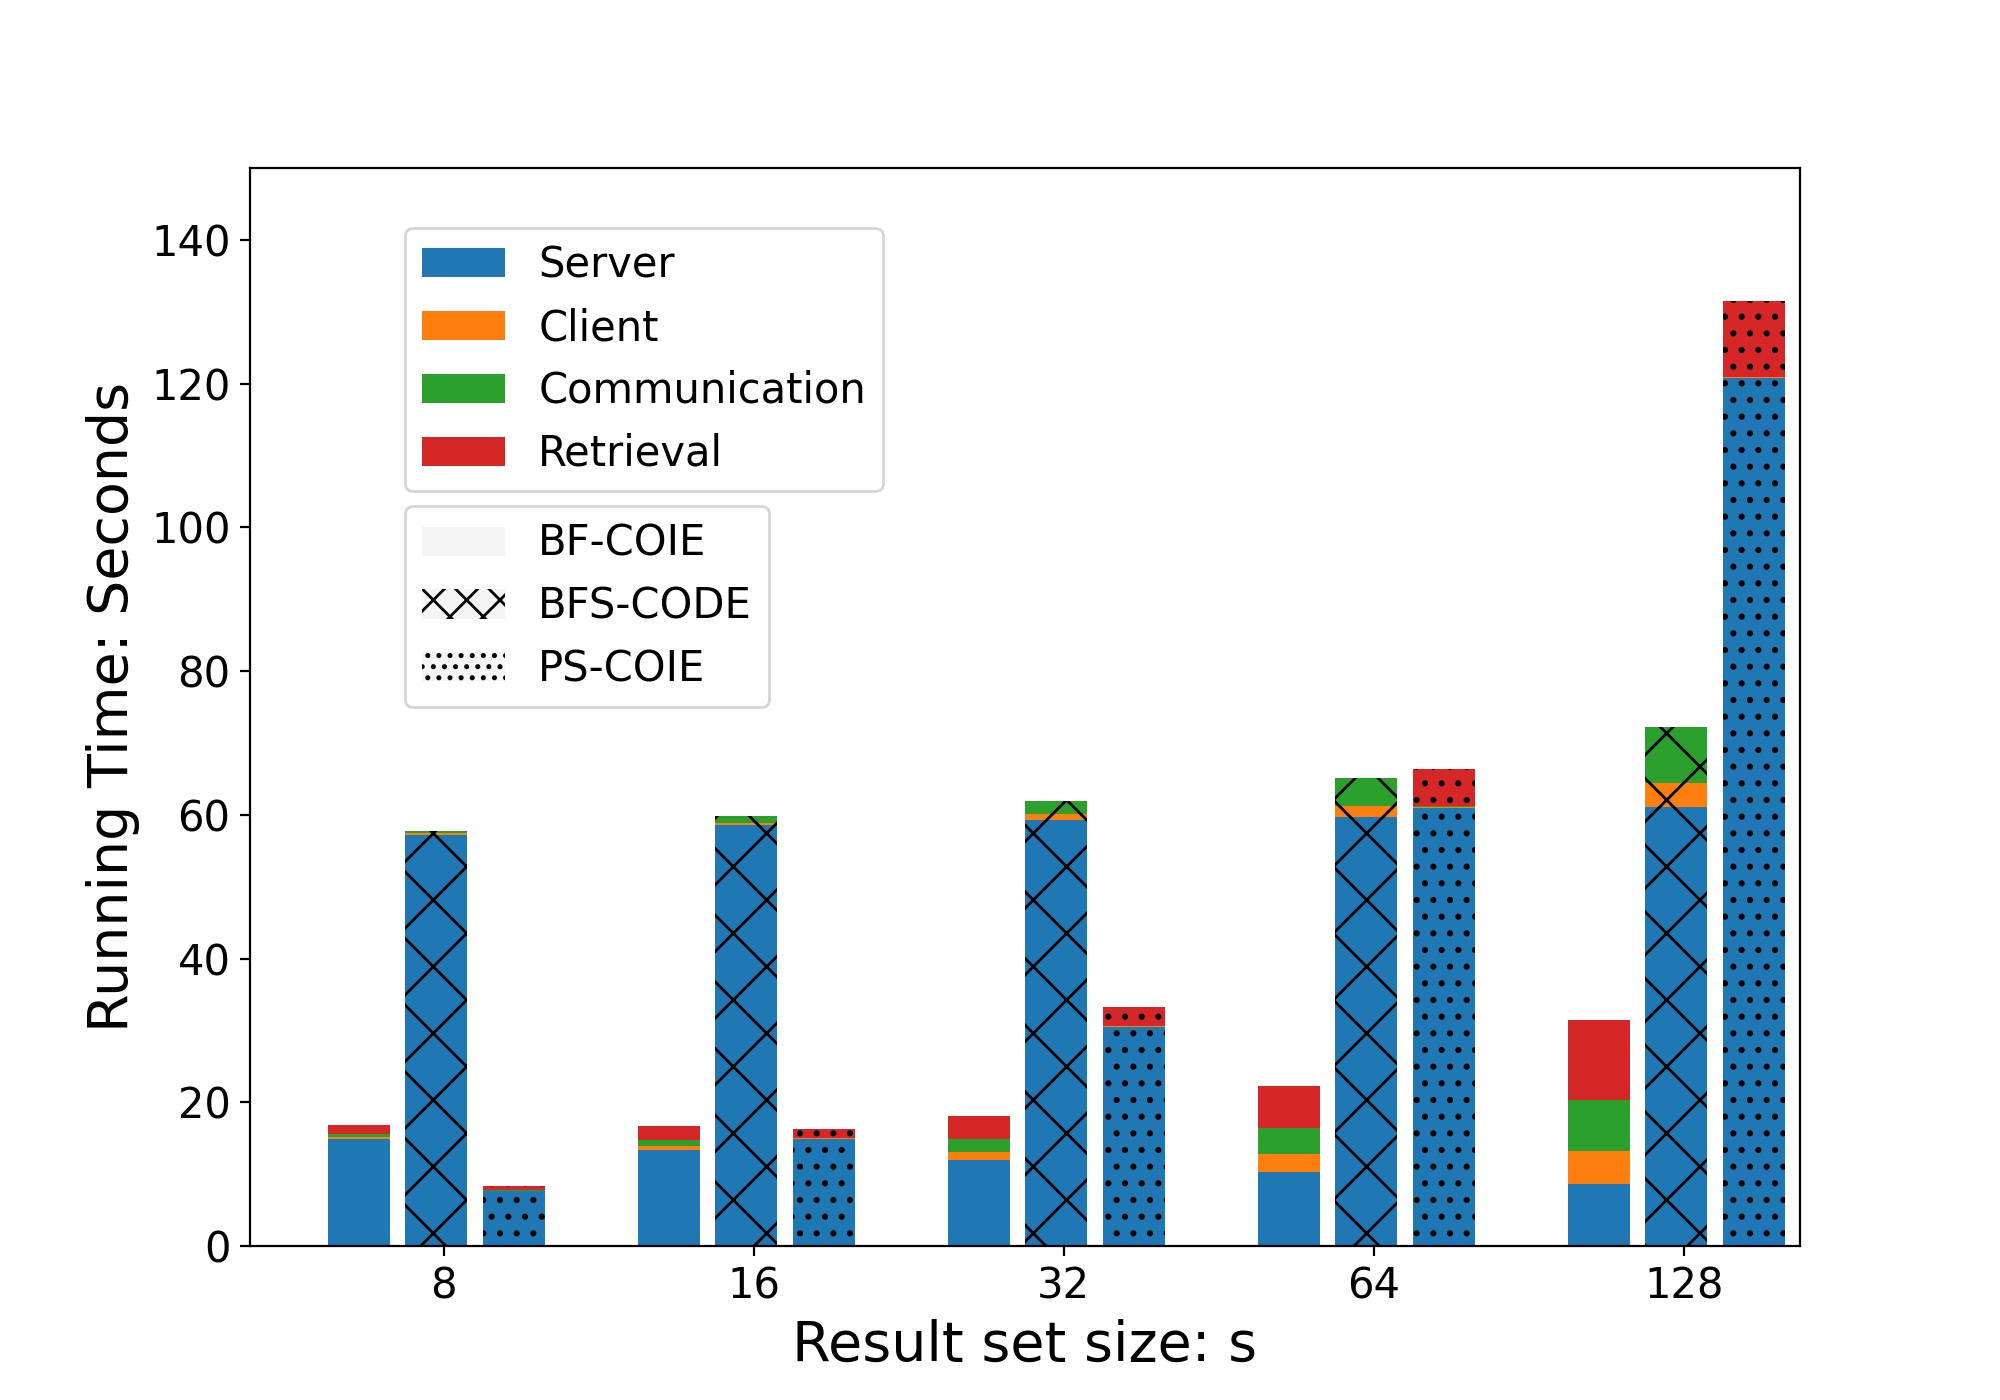
\includegraphics[width=.95\linewidth]{src/securesearch/expimgs/Figure_S.png}
\vspace{-1em}
\caption{Fetch time vs.~Result set size with $n=10,000$.}
\label{fig:ct_s}
\vspace{-1em}
\end{figure}

\paragraph{Results: fetch time vs.~the result set size.}
Figure~\ref{fig:ct_s} shows the performance of our protocols as a
function of the result set size $s$ while $n$ is fixed to $10,000$.
Here, again the performance is dominated by the encoding step, but the
relative costs have changed.  Due to the need to compute more power
sums, the PS-COIE protocol performs worse than BS-COIE and BFS-CODE when
$s$ becomes moderately large.  %Additionally, we can see that the
%client's cost of decoding in BFS-CODE grows linearly with the number of
%records to retrieve.  

The time used for transmitting the data over network (green in
Figure~\ref{fig:ct_s}) increases for larger $s$. However, it still
remains small for all three schemes.
%Given that the client can start decoding while downloading the
%ciphertexts without extra computation cost, the communication cost can
%be reduced even further. 
In the scenario of having lower network bandwidth, batching is
recommended to pack a vector of ciphertexts into a single ciphertext
with relatively low computation overhead. We discuss communication costs
further in Section~\ref{sec:comm}. 
%\lins{I edited this part, please make any change or fix. }


\subsubsection{Overall Running Time}

Although we do not optimize the Match step itself over prior work, we provide
an estimated comparison of the running time for the end-to-end flow.

Our search framework improves the overall search time by executing the Match
step only once, while the LEAF protocol must execute the Match step $s$ times.
Based on this, we can extrapolate the running time as follows: 

\BI
\item The overall running time for LEAF: 
$$ Time({\sf LEAF}) = s \cdot {\sf MT}({\sf LEAF})
  + s \cdot {\sf FT}({\sf LEAF}).$$ Here, $\sf MT$ and $\sf FT$ denote the
  match time and fetch time respectively. 

\item The overall running time for the BF-COIE scheme: $$Time({\sf
BF\mbox{-}COIE}) = {\sf MT}({\sf BF\mbox{-}COIE})
  + {\sf FT}({\sf BF\mbox{-}COIE})$$
\EI

Although the implementation (nor the algorithm) of the matching step of
LEAF protocol is not available in~\cite{CCS:WYXZ20}, we expect that it
holds 
${\sf MT}({\sf LEAF}) \approx {\sf MT}({\sf BF\mbox{-}COIE})$. 
%
In the experiment performed in LEAF (see Figure 9 in~\cite{CCS:WYXZ20}),
we have $m = \frac{ {\sf MT}({\sf LEAF})}{{\sf FT}({\sf LEAF})} \approx
1.5$.
%
For $s=16$, setting $ {\sf FT}({\sf LEAF}) = 1800 \cdot {\sf FT}({\sf
BF\mbox{-}COIE})$ based on the above discussion, we can estimate the
speed-up as follows:
$$ \frac {Time({\sf LEAF})}{Time({\sf BF\mbox{-}COIE})} = \frac{ s \cdot (m + 1) } { m + 1/1800}.$$ 
Thus, with $s = 16$, we estimate that our BF-COIE scheme has roughly 26X end-to-end speed-up. 


\subsubsection{Communication} \label{sec:comm}
We now look at the communication required by each of our schemes and by LEAF+.
Figure~\ref{tbl:communication_new} shows the network cost of the
protocols when the result set size $s$ is 16 and the size of the
database is $n=10,000$.  
In our implementations, the length of an FHE ciphertext is
approximately 103KB and the communication cost of PIR is
approximately 369KB. 

\begin{figure}[h]
\small
\begin{tabular}{lcccc}
\hline 
& LEAF+ & BF-COIE & PS-COIE & BFS-CODE \\
\hline
\#ct's  & $704$ & $1323$ & $17$ & $1321$ \\
\#PIR & 0 & 32 & 16 & 0 \\
\hline
\#ct's (w/~batching) & $32$ & $2$ & $2$ & $2$ \\
\hline
\end{tabular}

\caption{The communication costs ($n=10,000$ and $s=16$).} 
\label{tbl:communication_new}
\end{figure}

To explain this table, we first need to explain how we determined the costs of LEAF+ and PIR.

\BI
\item {\it LEAF+.}
Since LEAF+ fetches each data item and the corresponding index one by
one, LEAF+ needs to 16 rounds of communication to retrieve 16 data
items. Worse yet, LEAF+ requires the client to send the index of the
previous match (requiring $\lg{n}$ bits) in his next query to ensure
correctness.  Finally, LEAF+ uses bitwise encryption requiring a
ciphertext for each bit of the encrypted communication.  Thus, in a
single round, the client must send $\lg n=14$ ciphertexts and the server
returns $16+\lg n = 30$ ciphertexts -- $16$ ciphertexts for returning
the matching data item, and $\lg n$ ciphertexts to return its index.
This amounts to 704 ciphertexts for fetching 16 items (excluding the
query).    

\item {\it PIR costs.}
We reduce the cost of PIR for the COIE-based schemes by making a slight modification.
In addition to storing the FHE-encrypted database, the server also stores a copy
of each record encrypted using a symmetric-key encryption scheme (resulting in much
shorter ciphertexts).  Then, in the PIR step, the client fetches this symmetrically encrypted ciphertext 
instead of the FHE-encrypted one.

%
We use SealPIR for our PIR protocol, which requires 368.6 KB per request.
We remark that a very recently introduced SealPIR+ takes 80KB per
request~(see Table~1 in~\cite{MulPIR}), using which we can reduce the
communication further.
\EI

We can now compare the communication costs based on rows 1 and 2 of
Figure~\ref{tbl:communication_new}.  We see that the communication of
BF-COIE and BFS-CODE are roughly twice that of LEAF+, while PS-COIE
requires almost 10X less communication.  The extra communication needed
by BF-COIE and BFS-CODE can likely be offset by the much lower round
complexity required by our protocol since the latency costs are likely
higher than the cost for the extra bandwidth.

\paragraph{Reducing communication using ciphertext batching.}
We now describe an optimization to significantly reduce the
communication of our protocols at the cost of slightly increased server
computation.  SEAL allows thousands of encrypted values to be packed
together into a single ciphertext.  This allows us to pack the
ciphertexts in all of our protocols into just one a single ciphertext to
be sent from the server to the client.  However, this does require the
server to do some additional computation to pack the ciphertexts prior
to sending them.  We experimentally measured this packing, and it requires
approximately 3 seconds on a single threaded machine.

LEAF+ can also take advantage of packing to reduce the communication of
their protocols.  However, since the results must be returned one at a
time, the best LEAF+ can do is to pack all ciphertexts that are sent in
each round, resulting in a total of 32 ciphertexts. 

We note that the cost of PIR is unchanged by this modification.  Thus,
with the packing optimization, the communication of BFS-CODE is roughly
1/16 of the communication needed by LEAF+, but BF-COIE and PS-COIE
require approximately 4X and 2X more communication than LEAF+
respectively when SealPIR is used; however, when SealPIR+ is used, both
schemes have slightly less communication than LEAF+.  

